\documentclass[12pt,a4paper]{report} 
\setcounter{tocdepth}{3}
\usepackage[utf8]{inputenc}
\usepackage[USenglish]{babel}
\usepackage{graphicx}
\graphicspath{ {images/} }
\title{Data Mining\\Final project report\\
	\large Implementation of a single classification algorithm and several algorithms for feature reduction.}
\date{June, 2015}
\author{Przemysław Piórkowski, Michał Dębski, Damian Hermanowski}\begin{document}
\maketitle 
\tableofcontents
\chapter{Introduction}
The project objective is to implement single classification algorithm and several algorithms for feature reduction. In the addition, developed algorithms have to be evaluated against chosen data set and classification method.

Basing on the document provided by project's Supervisor and the initial research the Team decided to implement three types of the feature reduction algorithms: Document Frequency Thresholding (DFT), Mutual Information (MI) and \({\chi}^2\) statistic (CHI). As a classification algorithm the k-nearest neighbors (kNN) method was chosen. The Team decided to use the C++ programming language for implementation purposes.

The source data set: SPAM E-mail Database, consists of 4601 instances of e-mails. Each e-mail is considered either as a spam or not. Classification is based on 57 continuous attributes denoting particular words and characters frequency as well as lengths of uninterrupted sequences of capital letters in a message. The data set does not have any missing attribute values.

\chapter{Algorithms implementation}
DFT thresholding is the simplest technique for attribute
reduction. Document frequency is the number of documents in
which a term occurs. Our implementation counts occurences of not null values of each attribute. It utilizes the training set for this step. After that a vector of frequencies is created. An attribute which frequency is below given threshold is filtered out for further classification steps. The basic assumption is that rare
terms are either non-informative for category prediction,
or not influential in global performance.



MI tries to measure the influence of existence of particular attribute/term on a given class value. If one considers the two way contingency table of a term t and a category c, where A is the number of times t and c co-occur, B is the number of time the t occurs without c, C is number of times c occurs without t, and N is the total number of documents, then the mutual information criterion between t and c is estimated using formula:

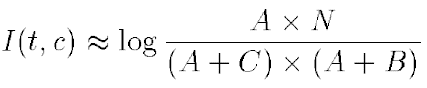
\includegraphics[scale=0.8]{MI1}

I(t ,c) equal to zero means that attribute/term t and category c are independent. The goodness of aterm/attribute is scored in two ways: as a average of MIs for a given attribute (MI\_AVG mode) and as a maximal MI for a given attribute (MI\_MAX mode). The outcome of the algorithm is a reduction vector of attributes scores. An attribute with a score below a given threshold is filtered out.

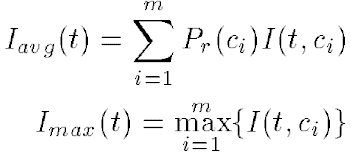
\includegraphics[scale=0.8]{MI_scores}



The \({\chi}^2\) statistic measures the lack of independence between an attribute t and a class c. Similarly to MI algorithm utilizes the two way contingency table with an additional value D, which equals to case when neither c nor t occurs. The term-goodness is calculated with a given formula:

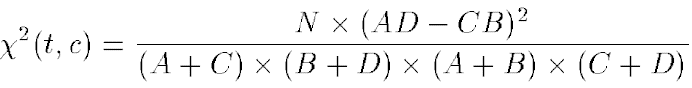
\includegraphics[scale=0.8]{CHI1}

Similarly to the MI method, the CHI statistic between the given attribute and classes may be computed as two scores: average value (CHI\_AVG mode) and maximum value (CHI\_MAX mode). The outcome of the algorithm is a vector of attributes scores. An attribute with a score below a given threshold is filtered out.

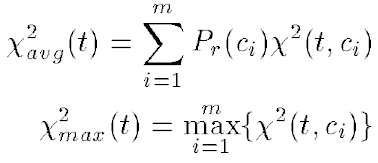
\includegraphics[scale=0.8]{CHI_scores}

The project implements three feature reduction algorithms within 3 classes:
\begin{itemize}
  \item CHIReduction
  \item DFTReduction
  \item MIReduction
\end{itemize}
The kNN algorithm is implemented in the \textbf{KNNClassifier} class. There were developed additional classes for data loading and data interpretation: \textbf{DataLoader}, \textbf{Data}. \textbf{DataAdapter} class is used to iterate over data in function defined manner. There is the \textbf{Logger} class for debugging and echoing purposes. There is the class supporting multithreading  for parallelization capabilities: \textbf{ParallelExecutor} with a support of \emph{AtomicIfPossible} and \emph{AtomicInternal} classes.

The developed project application can be run with given parameters:
\begin{itemize}
  \item \texttt{-ftrain trainFileName} - csv file name containing train dataset
  \item \texttt{-ftest testFileName} - csv file name containing test dataset
  \item \texttt{-h [TRUE,FALSE]} - switch for reading headers of a source file
  \item \texttt{-cname className} - class attribute header
  \item \texttt{-k value}
  \item \texttt{-CV value} - number of iterations/folds of cross valdiation
  \item \texttt{-DFT dftThreshold} - treshold for DFT algorithm
  \item \texttt{-MI\_MAX} - switches on MAX score calculation for MI algorithm
  \item \texttt{-MI\_AVG} - switches on AVG score calculation for MI algorithm
  \item \texttt{-MI miThreshold} - treshold for MI algorithm
  \item \texttt{-l verbosityLevel}  - value <1,5>
  \item \texttt{-CHI\_MAX}- switches on MAX score calculation for CHI algorithm
  \item \texttt{-CHI\_AVG}- switches on AVG score calculation for CHI algorithm
  \item \texttt{-CHI chiThreshold} - treshold for CHI algorithm
\end{itemize}

\chapter{Experiments}

In order to validate implemented algorithms against the data set the \emph{7-fold Cross-validation} method was used (\texttt{-CV 7}). kNN implementation has one control parameter - the number of neighbors voting. For evaluation purposes this k-value was set to 5.
The influence of each feature reduction algorithm on the kNN classification method was measured with precission and recall values. Scores were calculated as a geometric mean of values obtained from each round of the cross validation.  These quality measures were compared with the results of classification without feature reduction. Number of attributes was controlled with picked threshold values.

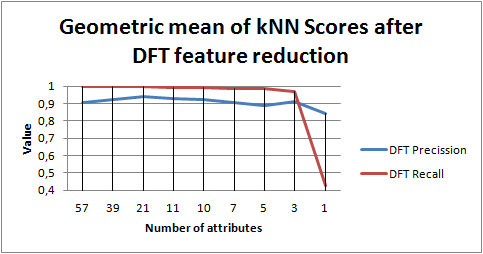
\includegraphics[scale=1]{DFTscores}

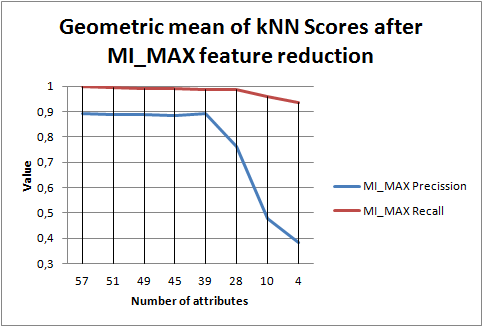
\includegraphics[scale=1]{MIMAXscores}

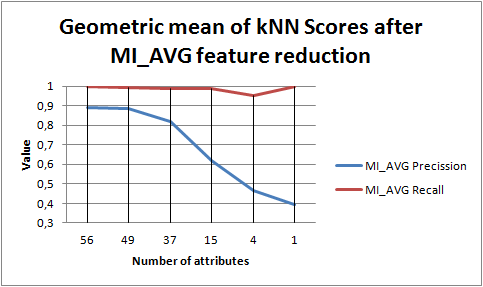
\includegraphics[scale=1]{MIAVGscores}

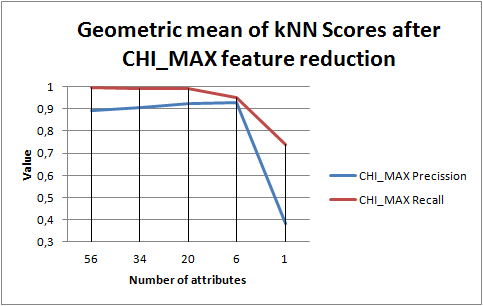
\includegraphics[scale=1]{CHIMAXscores}

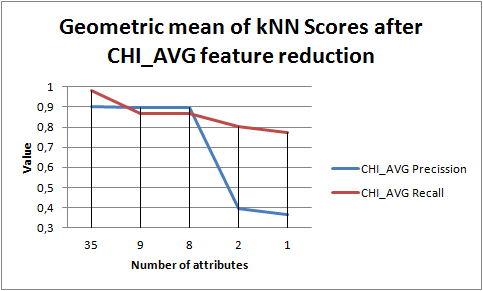
\includegraphics[scale=1]{CHIAVGscores}

\chapter{Conclusions}
The results are interesting. The application of DFT, CHI\_MAX and MI\_MAX on the given data set gave slight precission gain when less than a half of attributes were cut. The DFT method achieved high precission and recall scores even with 3 attributes left - it is a great result for a such simple algorithm. CHI\_MAX and CHI\_AVG methods marked comparable - good overall results. Mutual Inforamtion (MI) methods showed worse results for aggresive feature reduction.

\end{document}